% !TeX root = ./dissertation.tex
% !TeX spellcheck = en-GB
% REMEMBER: You must not plagiarise anything in your report. Be extremely careful.

\documentclass{l4proj}

    
%
% put any additional packages here
%
\usepackage{float}

% Referencing 
\usepackage[backend=biber,bibstyle=apa,citestyle=apa]{biblatex}
\DeclareLanguageMapping{british}{british-apa}
\bibliography{l4proj.bib}

% break bilbatex reference URL on number
\setcounter{biburlnumpenalty}{9000}

\usepackage{csquotes}


% license
\usepackage[
    type={CC}, 
    modifier={by-nc-sa},
    version={4.0},
]{doclicense}
 


\begin{document}

%==============================================================================
%% METADATA
\title{Why is This Sensitive? \\ Visualising Important Sensitivity Classification Features}
\author{Guillaume de Susanne d'Epinay}
\date{\today}

\maketitle

%==============================================================================
%% ABSTRACT
\begin{abstract}
    Every abstract follows a similar pattern. Motivate; set aims; describe work; explain results.
    \vskip 0.5em
    ``XYZ is bad. This project investigated ABC to determine if it was better. 
    ABC used XXX and YYY to implement ZZZ. This is particularly interesting as XXX and YYY have
    never been used together. It was found that  
    ABC was 20\% better than XYZ, though it caused rabies in half of subjects.''
\end{abstract}

%==============================================================================

% EDUCATION REUSE CONSENT FORM
% If you consent to your project being shown to future students for educational purposes
% then insert your name and the date below to  sign the education use form that appears in the front of the document. 
% You must explicitly give consent if you wish to do so.
% If you sign, your project may be included in the Hall of Fame if it scores particularly highly.
%
% Please note that you are under no obligation to sign 
% this declaration, but doing so would help future students.
%
%\def\consentname {My Name} % your full name
%\def\consentdate {20 March 2018} % the date you agree
%

\def\consentname{Guillaume de Susanne d'Epinay}
\def\consentdate{\today}

\educationalconsent


%==============================================================================
\tableofcontents

%==============================================================================
%% Notes on formatting
%==============================================================================
% The first page, abstract and table of contents are numbered using Roman numerals and are not
% included in the page count. 
%
% From now on pages are numbered
% using Arabic numerals. Therefore, immediately after the first call to \chapter we need the call
% \pagenumbering{arabic} and this should be called once only in the document. 
%
% Do not alter the bibliography style.
%
% The first Chapter should then be on page 1. You are allowed 40 pages for a 40 credit project and 30 pages for a 
% 20 credit report. This includes everything numbered in Arabic numerals (excluding front matter) up
% to but excluding the appendices and bibliography.
%
% You must not alter text size (it is currently 10pt) or alter margins or spacing.
%
%
%==================================================================================================================================
%
% IMPORTANT
% The chapter headings here are **suggestions**. You don't have to follow this model if
% it doesn't fit your project. Every project should have an introduction and conclusion,
% however. 
%
%==================================================================================================================================
\chapter{Introduction}

% reset page numbering. Don't remove this!
\pagenumbering{arabic}

\section{The need for Technology Assisted Sensitivity Review}



Motivations
why senstivity review
why technological problem



\section{Objectives}



\section{overview}

bulle tpoi t of chapter ocntent


%==================================================================================================================================
\chapter{Background}

need for explanations in ML

CITE SOME WORKS

\section{Literature Review}

\subsection{Technology Assisted Sensitivity Review}


\autocite{de_rijke_towards_2014} A first implementation of Machine Learning classifier for sensitivity Review

\autocite{mcdonaldUsingPartofSpeechNgrams2015} Improving classification with Part of Speech tagging

\autocite{jose_enhancing_2017} Improving classification with word embeddings

\autocite{pasi_active_2018} Active Learning ("loopback learning") implemeting reviewer feedback in Sensitivity prediction

\autocite{mcdonaldHowSensitivityClassification2019} User study with Machine Learning classification

CITE SOME GENERAL ML EXPLANATIONS PAPERS

\subsection{``Predictive Coding'' or \textit{TAR} for legal electronic discovery}

Ongoing research in the area of Judicial practice has applied the concept of TAR to the process of legal discovery. 
This research has coined the term ``Predictive Coding'' \autocite{carrollGrossmancormackGlossaryTechnologyassisted2013} as an industry specific use of TAR in the legal practice, particularly for ``legal discovery'', the pre-trial exchange of evidence by both parties. 

\textcite{grossmanTechnologyAssistedReviewEDiscovery2010} compared the performances of a manual and TAR aided eDiscovery process with data from the various teams of the TREC 2009 Legal Track \autocite{hedinOverviewTREC2009}. They conclude that TAR methods lead to more accurate eDiscovery relevance estimations with significantly lower effort than with an exhaustive manual discovery process.


One of these teams, \textcite{cormackEvaluationMachinelearningProtocols2014}, constructed various training sets for a given list of discovery topics from a corpus of eDiscovery documents using IR techniques (a search engine). They then fitted Logistic regression classifiers on these training sets to classify the rest of the collection as relevant or not for each topic.


\subsection{Document visualization techniques}

and elaborate on why didnt choose them
"people have done this"

\section{Related products}

Quite a few official government guidelines on the redaction of sensitive documents mention Adobe Acrobat as a go to tool for redacting text documents \autocite{thenationalarchivesRedactionToolkitPaper2016}. 
Sometimes, the guidelines \textit{are} Adobe's guidelines for redaction \autocite{scottishgovernmentRedactingInformation2019}.

\subsection{PDF editors}

Adobe Acrobat is a well known PDF toolkit that notably enables sensitivity redaction of documents. 
The principle is common: select text, click redact and browse a nested context menu to select an exemption (Figure \ref{fig:adobe-redaction}).

\begin{figure}[H]
    \centering
    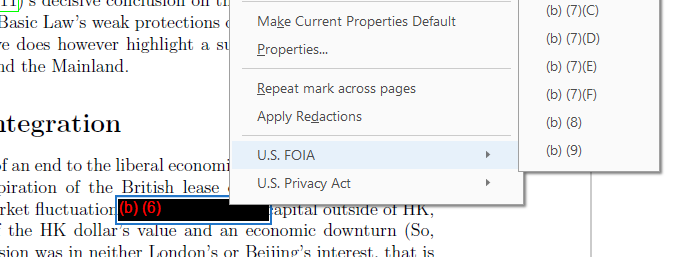
\includegraphics[width=\linewidth]{images/adobe_redaction.png}
    \caption{Adobe Acrobat redaction workflow}
    \label{fig:adobe-redaction}
\end{figure}

There are a variety of PDF editors, when they implement document redaction, they closely resemble this workflow. 
For instance, Foxit PhantomPDF is another well known PDF editor that implements a strikingly similar context menu (Appendix \ref{fig:foxit-menu}) also allows for document wide redaction of a text selection (Appendix \ref{fig:foxit-redact-all}), something which Adobe implement quite poorly (Appendix \ref{fig:adobe-redact-all}).

%==================================================================================================================================
\chapter{Requirements}

\section{Scope}

\section{(non)Functional definition}

user study

\section{Wireframes}

\begin{figure}
    \centering
    \begin{subfigure}[b]{\linewidth}
        \centering
        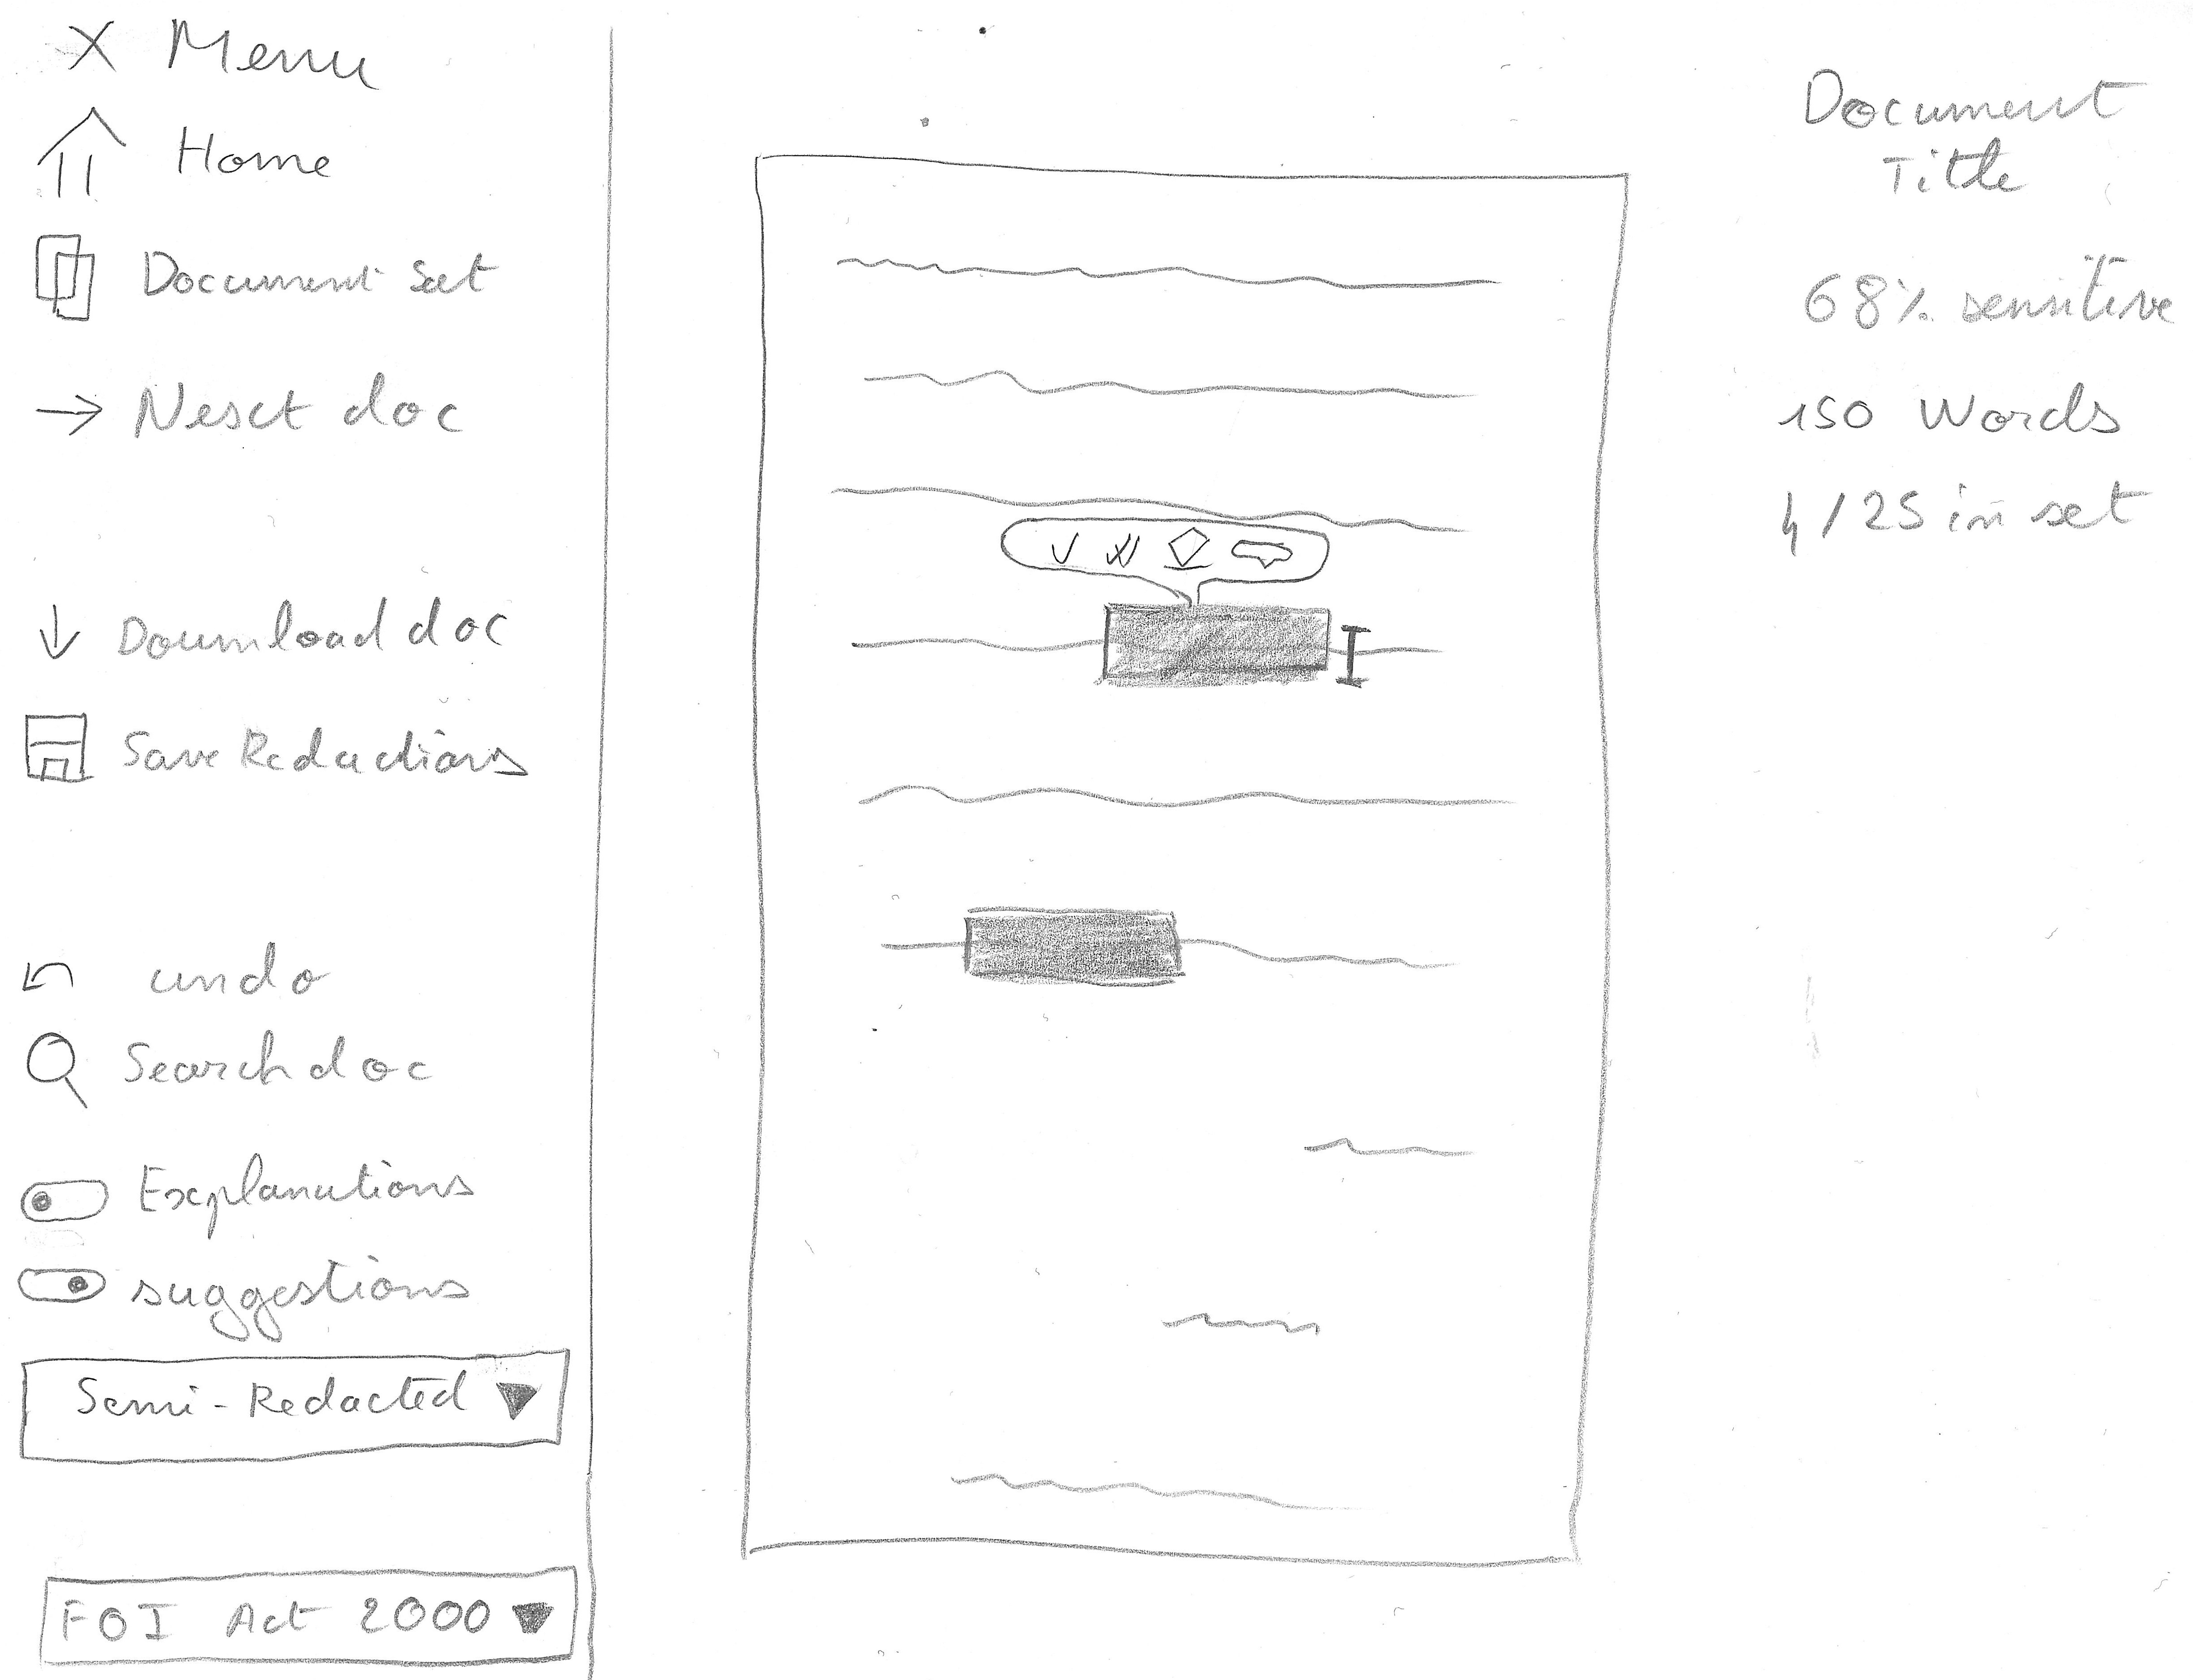
\includegraphics[width=0.6\linewidth]{images/wireframe_doc_view.jpg}
        \caption{Document View Wireframe}
        \label{fig:document-wireframe}
    \end{subfigure}
    \begin{subfigure}[b]{\linewidth}
        \begin{subfigure}[b]{0.5\linewidth}
            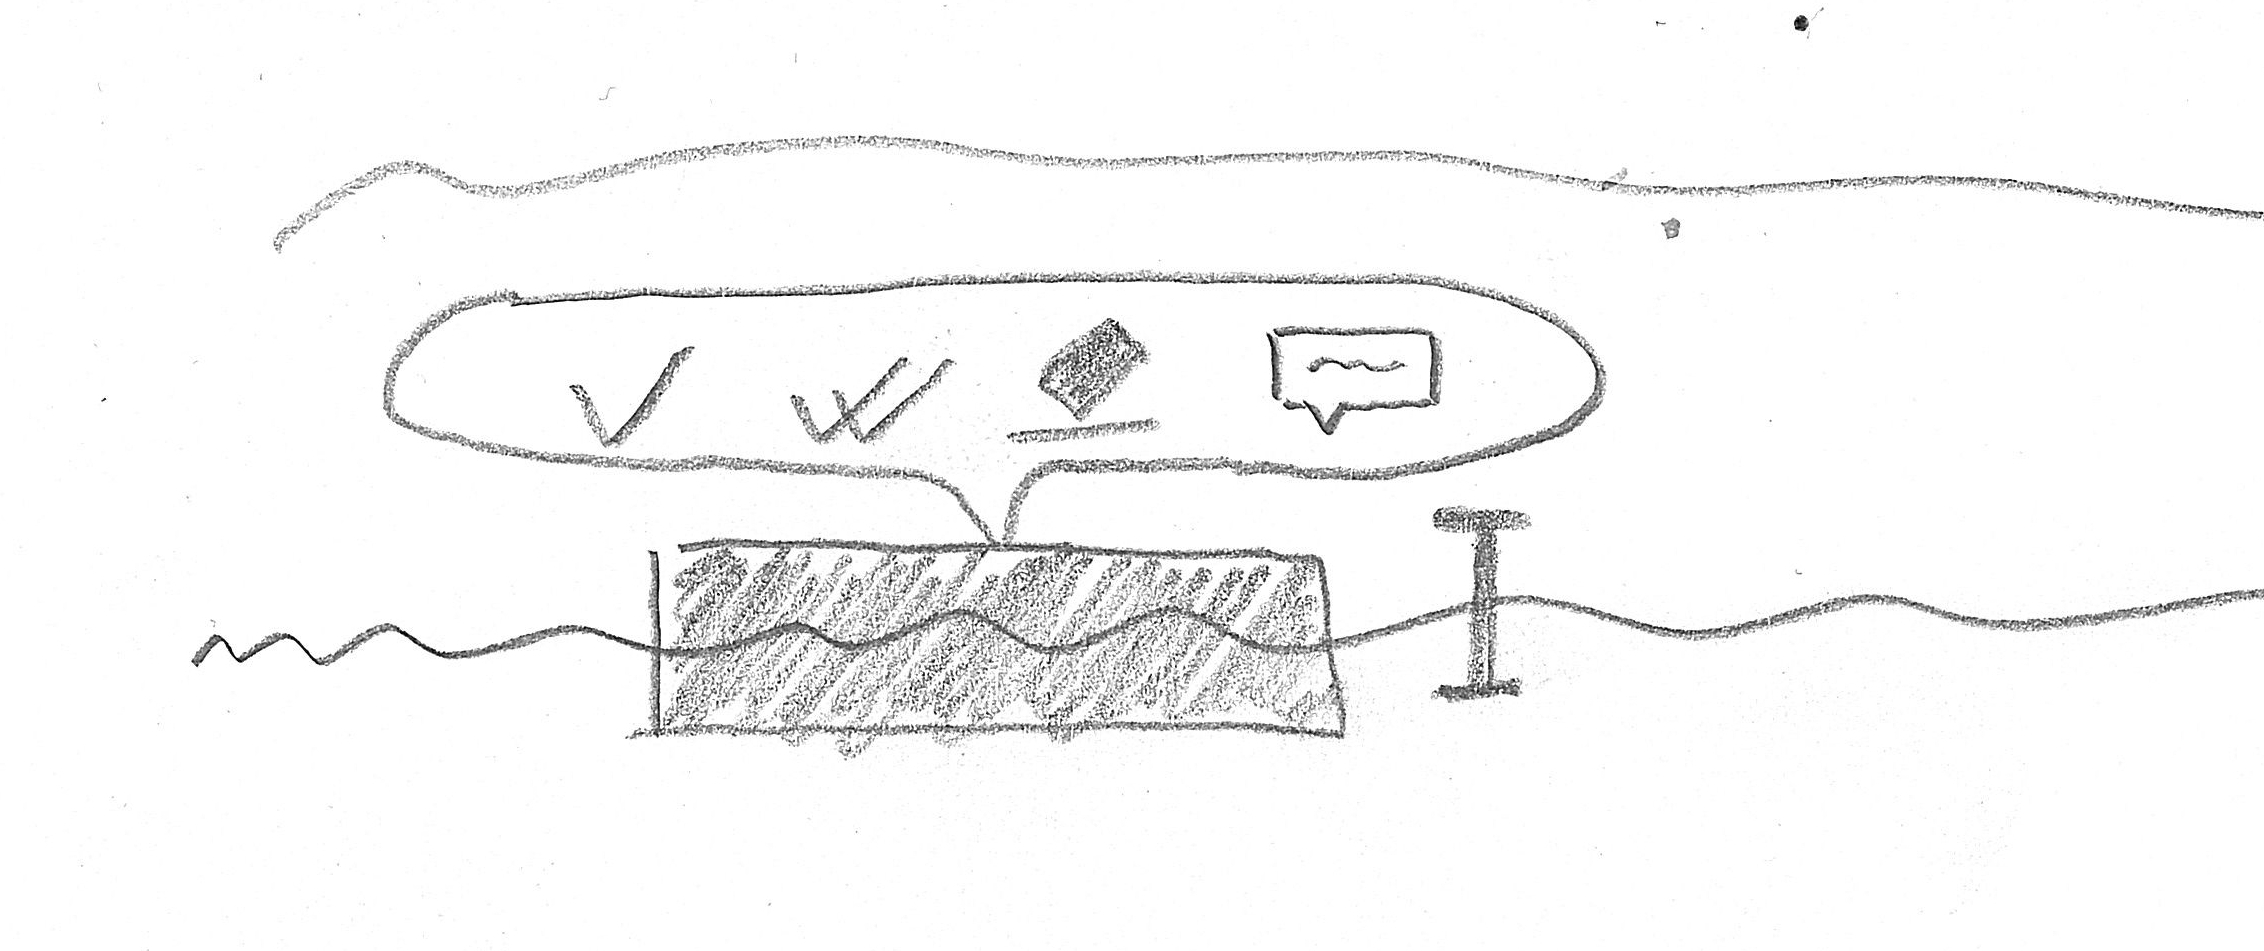
\includegraphics[width=\linewidth]{images/wireframe_tooltip.jpg}
            \caption{minimized tooltip wireframe}
            \label{fig:tooltip-wireframe}
        \end{subfigure}
        \begin{subfigure}[b]{0.4\linewidth}
            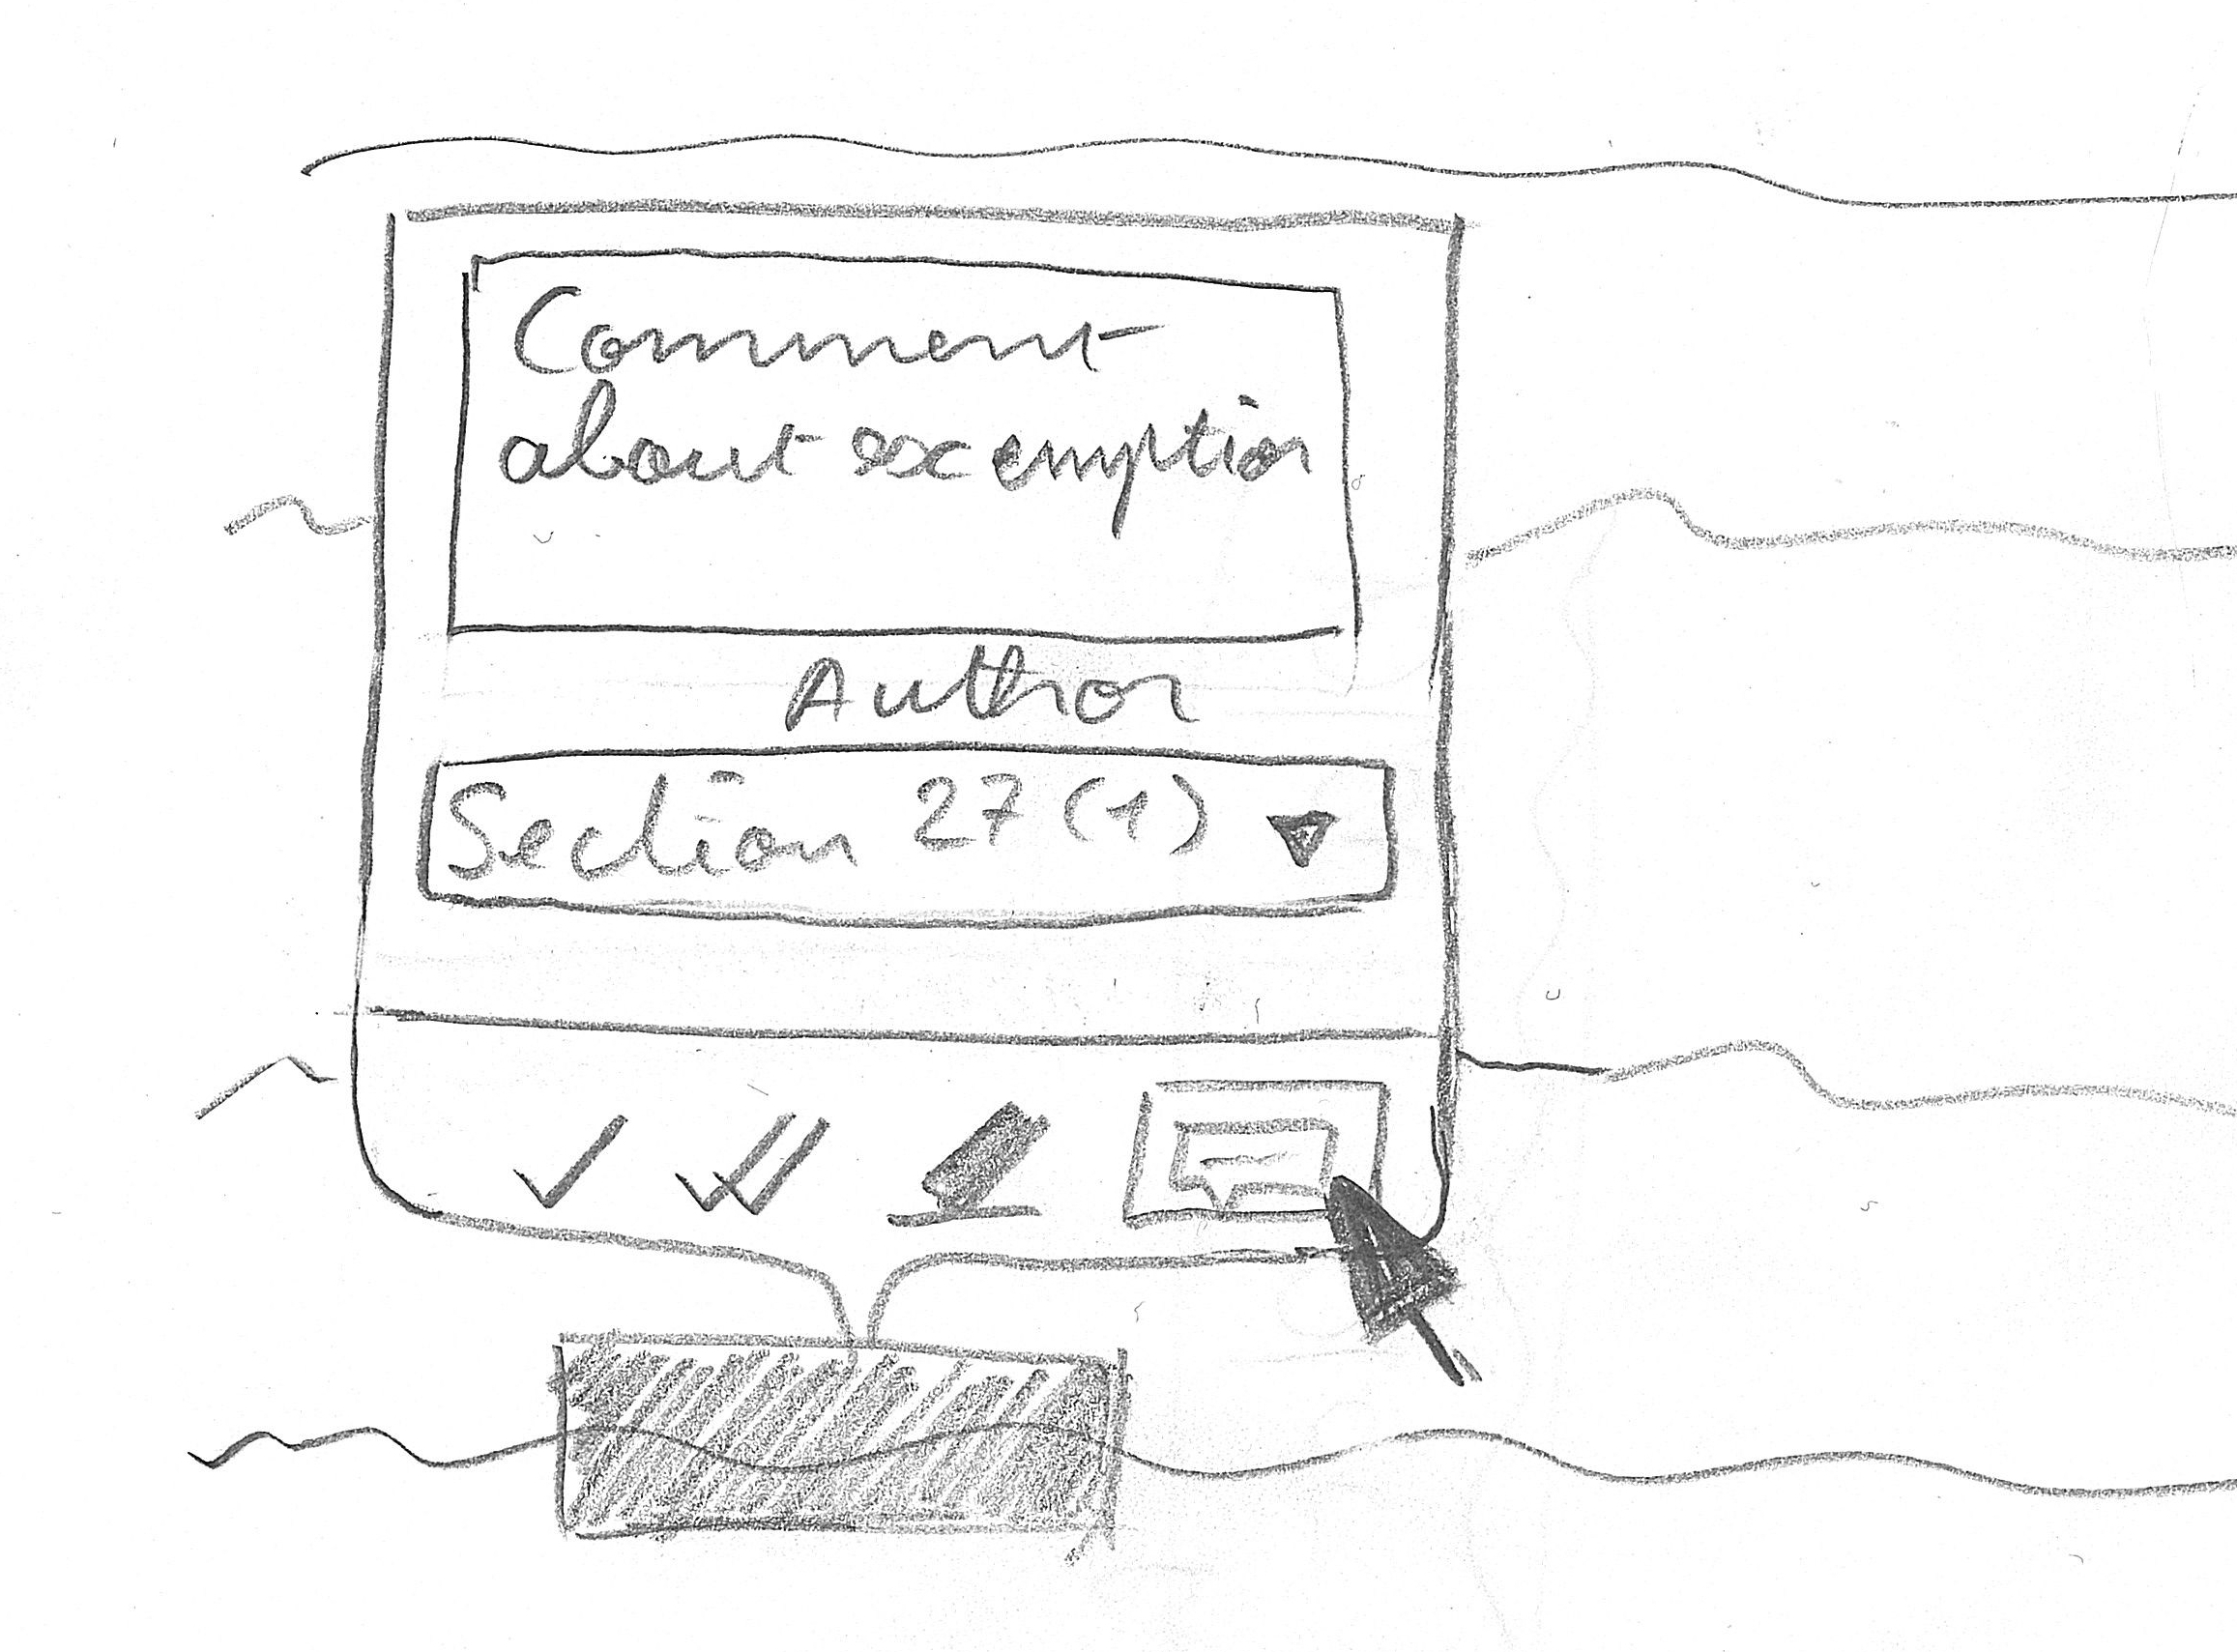
\includegraphics[width=\linewidth]{images/wireframe_tooltip_comment.jpg}
            \caption{Expanded tooltip wireframe}
            \label{fig:expanded-tooltip-wireframe}
        \end{subfigure}
    \end{subfigure}
    \caption{Selection of some of the Wireframes drawn up during the design process}
    \label{fig:wireframes}
    
\end{figure}


%==================================================================================================================================
\chapter{Design}

link back to requirements

choice of technologies

\section{Application Structure and Technology stack}

\section{Machine Learning Model}

% TODO this sounds too much like a list
To create the Machine Learning model for sensitivity classification, I have used the renowed Scikit-Learn Python framework from \textcite{pedregosaScikitlearnMachineLearning2011}.
For performance reasons, I later replaced its SVC implementation with a drop-in parrallelized replacement called ThunderSVM which can operate on multicore CPUs or CUDA enabled GPUs \autocite{wenThunderSVMFastSVM2018}.
I was able to resample my highly unbalanced dataset using the imblearn sampling library which extends Scikit-Learn \autocite{lemaitreImbalancedlearnPythonToolbox2017}.

% TODO elaborate on this
Then, in order to explain the model's predictions to the reviewer, I explored the Lime Framework, which calculates feature weights by toggling feature on or off to calculate their contributions to the prediction \autocite{ribeiroWhyShouldTrust2016a}.

% TODO 
\autocite{lundbergUnifiedApproachInterpreting2017a} Shapley values

\section{API}

\section{Frontend}

%==================================================================================================================================
\chapter{Implementation}

show coponennt code and how it gets data from backend

show lime explanations generation

key ``features'' code overview


\begin{itemize}
    \item Hands on SkLearn framework, experimented with different text pre-processing techniques and classifiers to build a Pipeline to classify textual documents into either sensitive or not sensitive categories
    \item overview of Machine Learning model explanation techniques, successfully implemented the Lime explainer, tried to use the SHAP explainer, but was unsuccessful
    \item Explore text document storage, looked at Terrier, ElasticSearch to finally settle on MongoDB
    \item Packaged SkLearn classifier into Python Flask API with OpenAPI specification
    \item created Javascript API Client from code generated from OpenAPI specification
    \item hands on ReactJS Javascript frontend framework, implemented a document browsing, viewing and upload frontend
    \item added text redaction feature to mark sections as sensitive with a label explaining why it is deemed sensitive
    \item implemented Lime Model explanations in Python backend, exposed them to the Flask API and created a frontend "in text" visualization of these sensitivities
    \item Research Document visualization techniques (literature review)
    \item created a populator script to load and classify all documents
    \item graph visualization of feature contribution to the classification and other UI tweaks
\end{itemize}

%==================================================================================================================================
\chapter{Evaluation}

We conducted a user evaluation in order to evaluate the effectiveness of our application in helping reviewers conduct a sensitivity review. We sought to answer a handeful of research questions.

\begin{itemize}
    \item Firstly, does our visualization of predicted document sensitivity and explanation features help reviewers conduct a sensitivity review faster?
    \item Secondly, does it improve the accuracy of the sensitivity review process.
    \item Lastly, does it improve reviewers' confidence in the completeness of their sensitivity review
\end{itemize}

\section{Preparations and Experimental Setup}

The collection is a set of 3801 Government documents relating to International Activities.
% TODO can you really say ground truth for sensitivity?
Our collection's ground truth for sensitivity was established with respect to sections 40 (International Relations) and 27 (Personal Information) of the Freedom of Information Act (FOIA).

An important consideration in the decisions that follow is that we did not have access to professional document reviewers, as such the evaluation was conducted with students in the role of reviewers. 
Out test reviewers were asked to identify sensitivities according to section 27 of the FOIA. Since our reviewers are not experts, thus finding Personal Information in a document is easier than identifying sensitivities harming International Relations (Section 40).
Due to time constraints we only selected short documents to show our reviewers, that is, documents under 2000 characters. 

We selected both sensitive and non-sensitive documents in order to represent every category of the confusion matrix for the classifier with the following counts:

\begin{table}[H]
    \begin{tabular}{l ll}
                                & Actually non-sensitive & Actually Sensitive \\ 
        Predicted non-sensitive & 3                      & 1                  \\
        Predicted Sensitive     & 1                      & 1                 
    \end{tabular}
    \caption{Document selection in the classifier's confusion matrix}
    \label{tab:confusion-matrix-selection}
\end{table}


Multiple interfaces were required to evaluate the effectiveness of the application.
One interface \textit{test mode 1} (Figure \ref{fig:test-mode-1}) is a simplified version of the final interface containing the classification prediction and the accompanying explanations.
The other, \textit{test mode 2} (Figure \ref{fig:test-mode-2}) is a stripped down version that only displays the document, and the manual redaction tools (document title and sensitivity type selection).

Our reviewers reviewed documents with both interfaces, the first interface displayed was chosen at random.


\begin{figure}[H]
    \centering
    \begin{subfigure}[b]{0.7\textwidth}
        \centering
        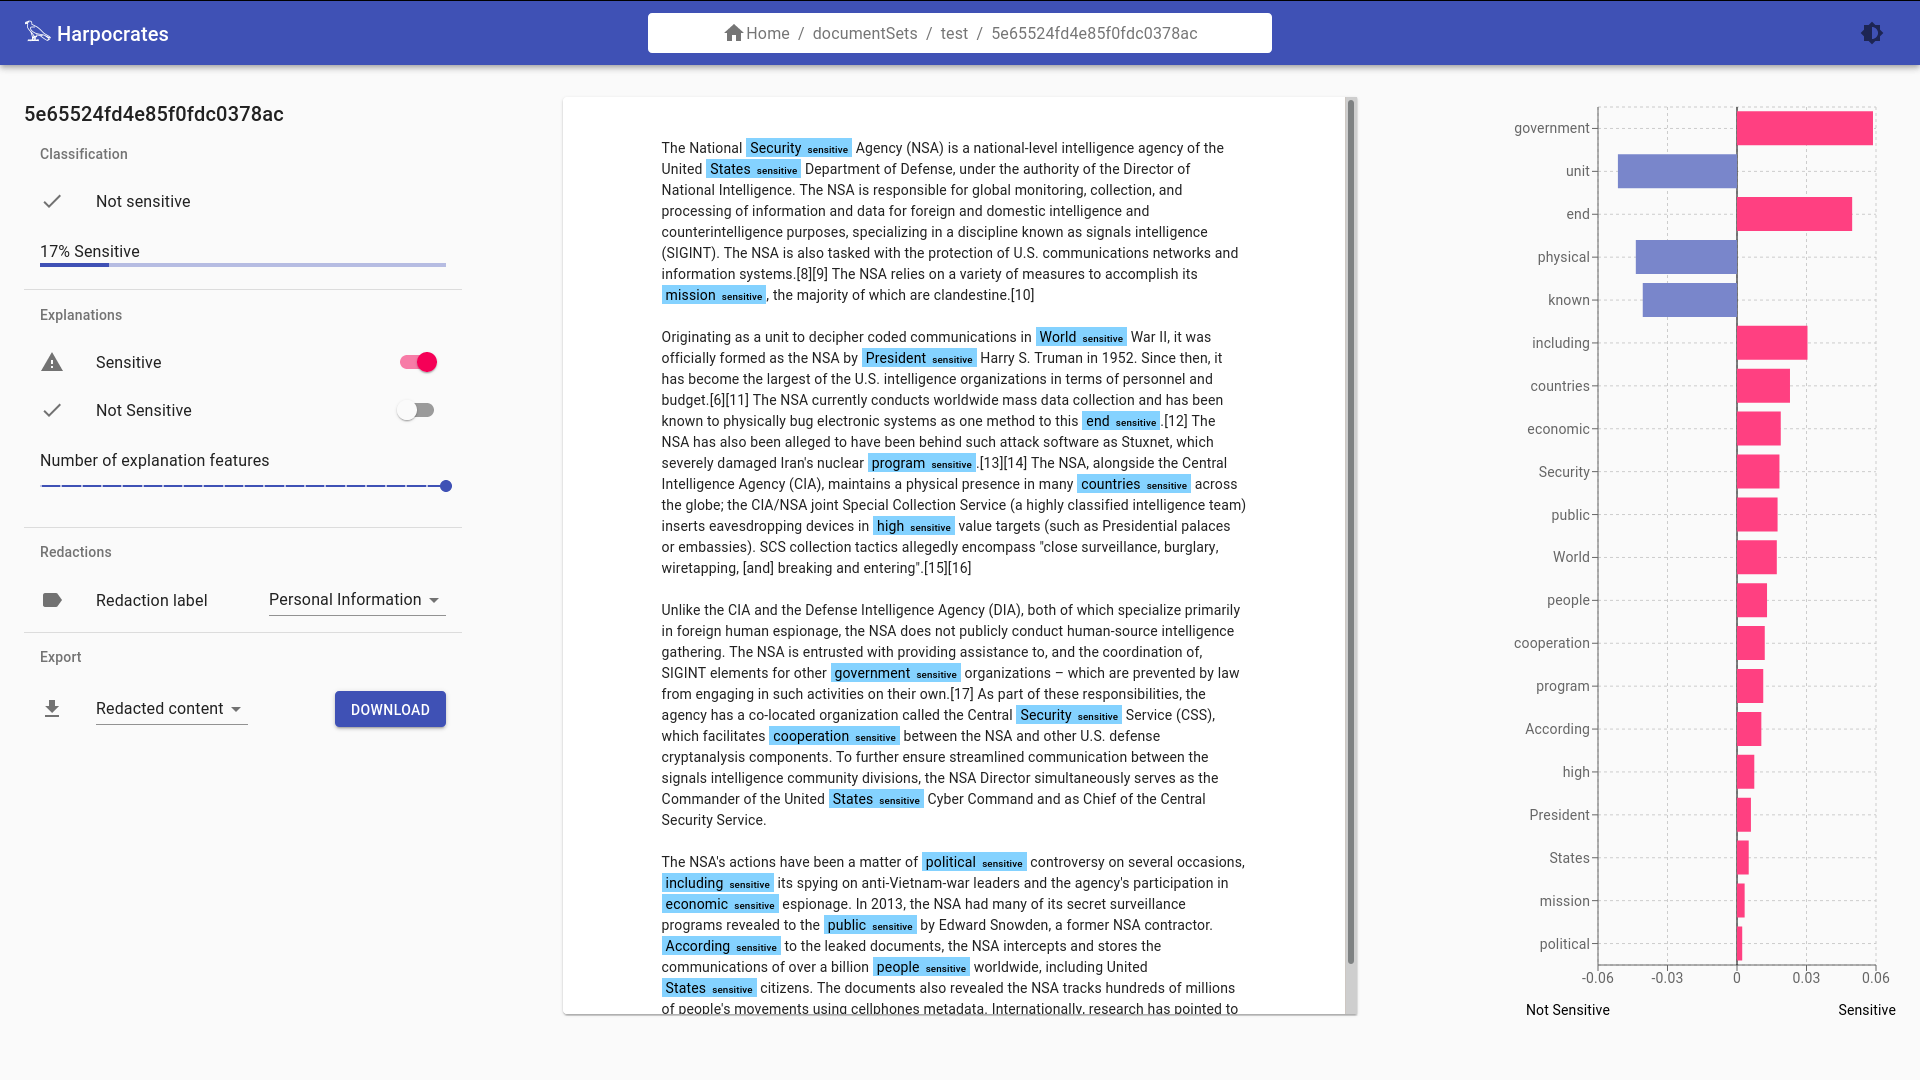
\includegraphics[width=\linewidth]{images/ui_test_mode_1.png}
        \caption{Test mode 1}
        \label{fig:test-mode-1}
    \end{subfigure}
    
    
    \begin{subfigure}[b]{0.7\textwidth}
        \centering
        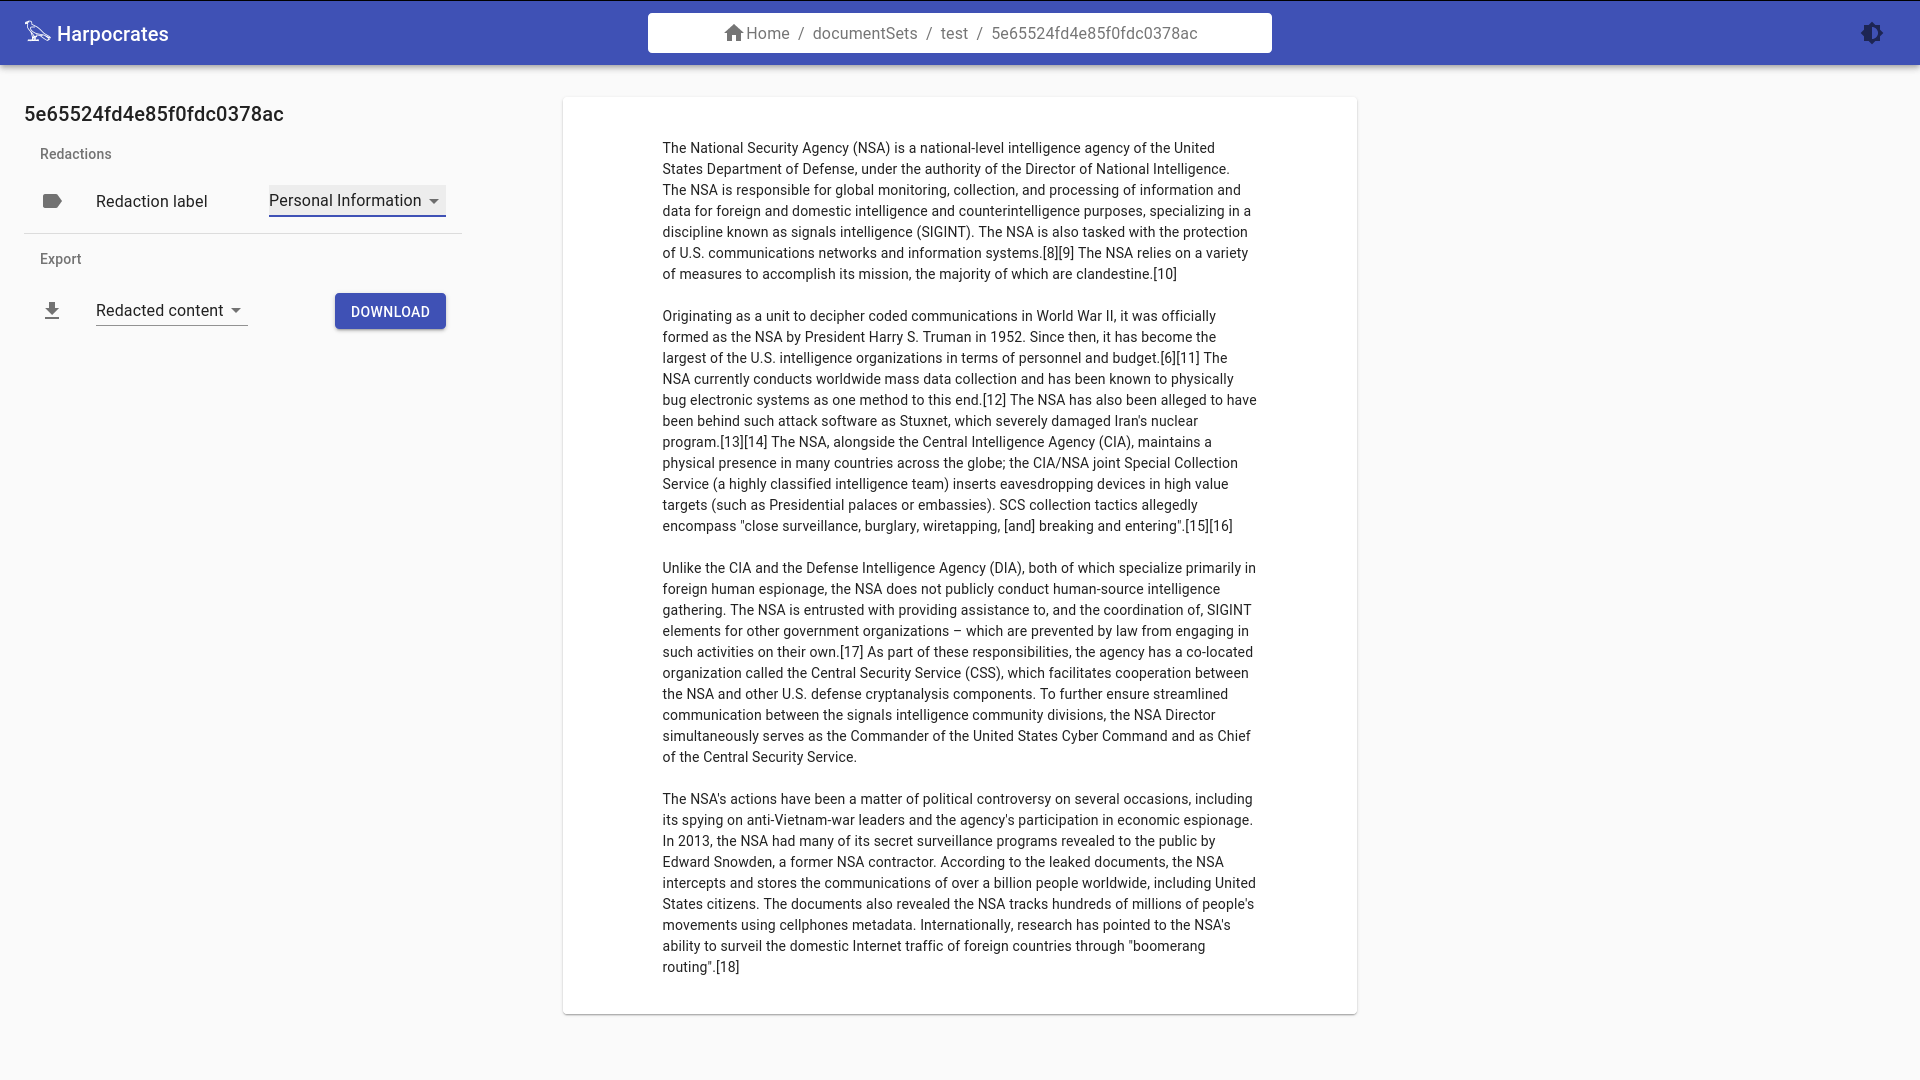
\includegraphics[width=\linewidth]{images/ui_test_mode_2.png}
        \caption{Test mode 2}
        \label{fig:test-mode-2}
    \end{subfigure}
    \caption{The two test modes used for evaluation}
    \label{fig:test-modes}
\end{figure}

% TODO put questionnaire in appendix 
% TODO link questionnaire here
Lastly, after the review of a batch of documents with each interface, a questionnaire was handed out to the testers

\section{Evaluation}

As mentioned, each user will be asked to review one collection of 6 documents for personal information sensitivities (FOIA Section 27) per user interface

The independent variables will a set of two user interfaces: with and without the predicted classification and explanations (more details below) which all users will both use. We will measure multiple dependent variables:

\begin{itemize}
    \item Firstly, we will measure the time to review an entire collection with each interface.
    \item Secondly we will record the accuracy of each reviewer on each interface for all documents.
    \item Lastly, we will evaluate the confidence of the reviewers after using each interface with a Likert scale in the questionnaires.
          
\end{itemize}




Research questions
dependent/indepdent variables
UI variations
experimental setup
document, subject seleciton


results


link back to requirements 
how have they been met
unit testing




%==================================================================================================================================
\chapter{Conclusion}


requirements I've met


reflections 

future work

%==================================================================================================================================
%
% 
%==================================================================================================================================
%  APPENDICES  

\begin{appendices}
    \chapter{PDF Editors}
    \section{PhantomPDF context menu}
    \label{fig:foxit-menu}
    \begin{figure}[H]
        \centering
        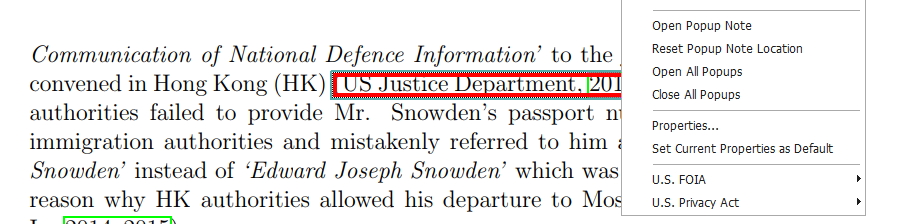
\includegraphics[width=\linewidth]{images/foxit_redaction.png}
    \end{figure}
    \section{PhantomPDF redact all}
    \label{fig:foxit-redact-all}
    \begin{figure}[H]
        \centering
        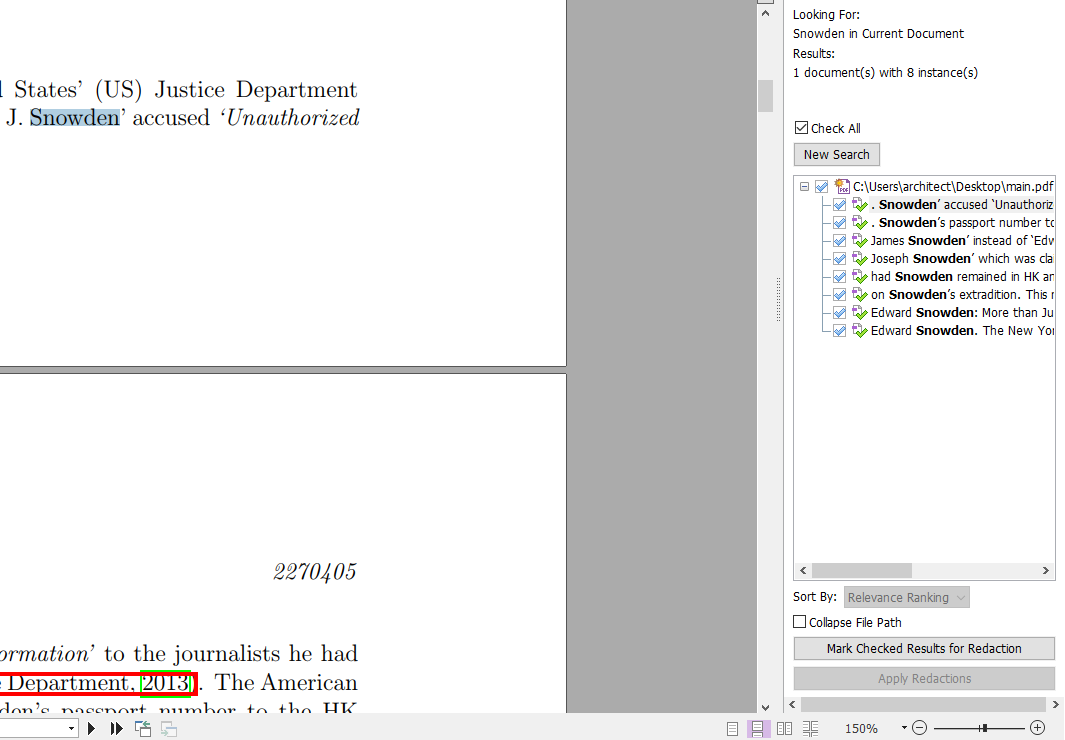
\includegraphics[width=\linewidth]{images/foxit_redact_all.png}
    \end{figure}
    \section{Adobe Acrobat redact all}
    \label{fig:adobe-redact-all}
    \begin{figure}[H]
        \centering
        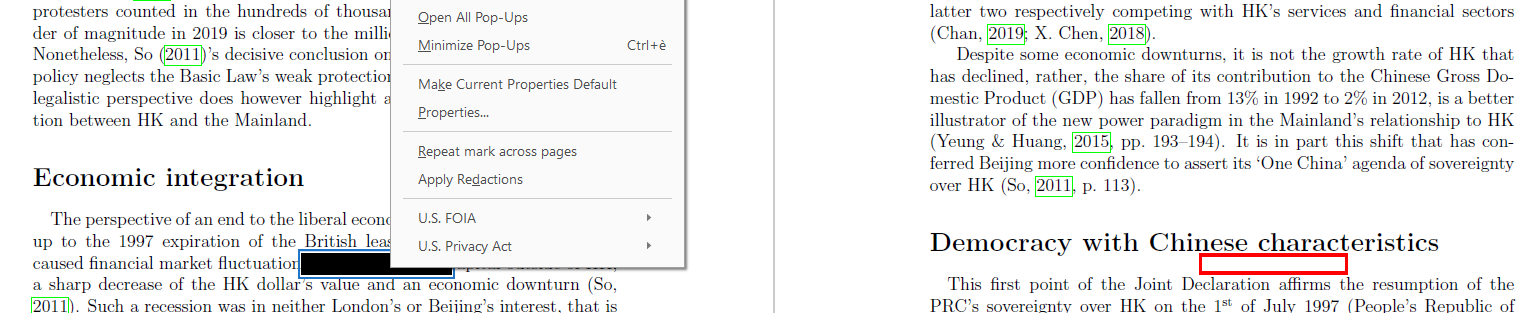
\includegraphics[width=\linewidth]{images/adobe_redact_all.png}
    \end{figure}
\end{appendices}
%==================================================================================================================================
%   BIBLIOGRAPHY   


\newpage


\section*{References}

\printbibliography[heading=none]

\vspace*{\fill}
% print license
\doclicenseThis

\end{document}
